\chapter{Application: Image Based Lighting}
\label{ch:application_ibl}
In this chapter we start by describing image based lighting shortly.
Following that the approach of Karl\'ik et al. is explained to use in image based lighting.
At the end we take look at the results from~\cite{Karlik2019}.
\todo{Explain the contents of this chapter (at the end)}


\section{Image Based Lighting}
\label{sec:ibl}
Creating realistic lighting for a scene can be very complex and time consuming.
To avoid modelling a lighting environment a commonly used method is to create an image of a real world environment
and using that for the direct illumination of a scene.
This approach is called image based lighting and was introduced back in 1998 by Debevec in~\cite{debevec}.\\
To get the lighting of a scene in the real world you could place a mirror sphere in the middle of your scene
and the a photo of that sphere ideally from far away
so the camera itself doesn't take up a large part of the scene.
This method is called sphere mapping.
During rendering you place your scene in the center of that textured sphere
and if a shadow ray doesn't hit any object of the scene you read out the texel
on the sphere that corresponds to the direction of the ray.\\
A different method is to take six pictures of the scene from the top, bottom, left, right, front and back
and then use the same evaluation method as with the sphere with the direction of the shadow ray direction
to get the texel from the environment map.
For more information on how to use environment maps/image based lighting consider~\cite{environment_map}.


\section{MIS Compensation in Image Based Lighting}
\label{sec:misc_ibl}
Here we will discuss the image based lighting application example from Karl\'ik et al. in~\cite[Section~6-7]{Karlik2019}.


\subsection{Setup}
\label{sec:ibl_setup}
They calculate the unoccluded direct illumination with the following rendering equation:
\begin{equation}
    \label{eq:ibl_render_equation}
    L_{dir}(x, \omega_o) = \int_{H(n)} L_I(\omega_i) \rho(x, \omega_i, \omega_o) |n \cdot \omega_i|_+ d\omega_i.
\end{equation}
$ x $ is the surface position and $ \omega_o $ the outgoing view direction.
The integration domain $ H(n) $ is the upper hemisphere centered around the normal $ n $.
The HDR environment map is used through $ L_I(w_i) $,
$ \rho(x, \omega_i, \omega_o) $ corresponds to the BRDF at position $ x $
with incoming direction $ \omega_i $ and outgoing direction $ \omega_o $.
$ |n \cdot \omega_i|_+ $ is the positive cosine of the angle between the normal and the incoming direction i.e. $ max\{0, |n \cdot \omega_i|\} $.\\
In a standard Monte Carlo renderer two pdfs would be used,
one proportional to the BRDF-cosine product and another one proportional to the environment map.
Those two would then be combined in MIS with the balance heuristic.
Generally the BRDF-cosine product pdf is given analytically and depends on the position, the outgoing and the incoming direction
whereas the environment map pdf is mostly tabulated and only depends on the incoming direction.
Since the second one is easier to modify,
that one was used as the free pdf in their work.


\subsection{PDF solutions}
\label{sec:ibl_pdfs}
To get the compensated pdf sampling technique equation~\ref{eq:ibl_render_equation}
and the BRDF sampling pdf $ p_{\rho}(x, \omega_i, \omega_o) $ are inserted into equation~\ref{eq:valid_compensated_pdf}
to get $$ \tilde{p}_I(x, \omega_i, \omega_o) = \frac{1}{b} max\{0, \frac{f_I(x, \omega_i, \omega_o)}{c_I L_{dir}(x, \omega_o)} - \frac{1 - c_I}{c_I} p_\rho(x, \omega_i, \omega_o)\} $$
where $ f_I(x, \omega_i, \omega_o) = L_I(\omega_i) \rho(x, \omega_i, \omega_o) |n \cdot \omega_i|_+ $,
$ c_I $ is the proportion of samples for the free pdf and b is the normalization factor to make it integrate to one.
Since this solution depends on the position, the incoming and the outgoing direction they proposed a simpler solution we will show in the upcoming section.


\subsubsection{Normal-dependent solution}
\label{sec:ibl_normal_dependent}
To remove the dependency on the position and the outgoing direction they assumed a Lambertian BRDF with albedo $ \rho \equiv \frac{1}{\pi} $
which yields:
\begin{equation}
    \label{eq:normal_dependent}
    p_I^{nd}(\omega_i, n) = \frac{1}{b_{nd}} max\{0, \frac{f_{nd}(\omega_i, n)}{c_I \int_{H(n)} f_{nd}(\omega, n) d\omega} - \frac{1 - c_I}{c_I} \frac{|n \cdot \omega_i|_+}{\pi}\}.
\end{equation}
This formula does depend on the surface normal,
but it can still be precomputed for a number of directions.
Since this solution is more practical than the more general one before it still might require changes in the rendering implementation.
Therefore they introduced one more solution that uses less memory and has even less dependencies.


\subsubsection{Normal-independent solution}
\label{sec:ibl_normal_independent}
This method averages over all normal directions (for a detailed explanation please refer to~\cite[Appendix~D]{Karlik2019})
to get a pdf that is only dependent on the incoming direction: $$ p_I^{ni}(\omega_i) = \frac{1}{b_{ni}} max\{0, L_I(\omega_i) - 2 (1 - c_I) \bar{L}_I\}. $$
As above $ b_{ni} $ is the normalization factor and $ \bar{L}_I $ is the average of the HDR map luminance.
If we look close we see that the formula corresponds to a simple subtraction from the complete environment map and then re-normalizing it.


\subsection{Evaluation}
\label{sec:ibl_evalution}
They used a simple 1D setup as shown in figure~\ref{fig:ibl_setup} for their empirical tests.

\begin{figure}[h]
    \centering
    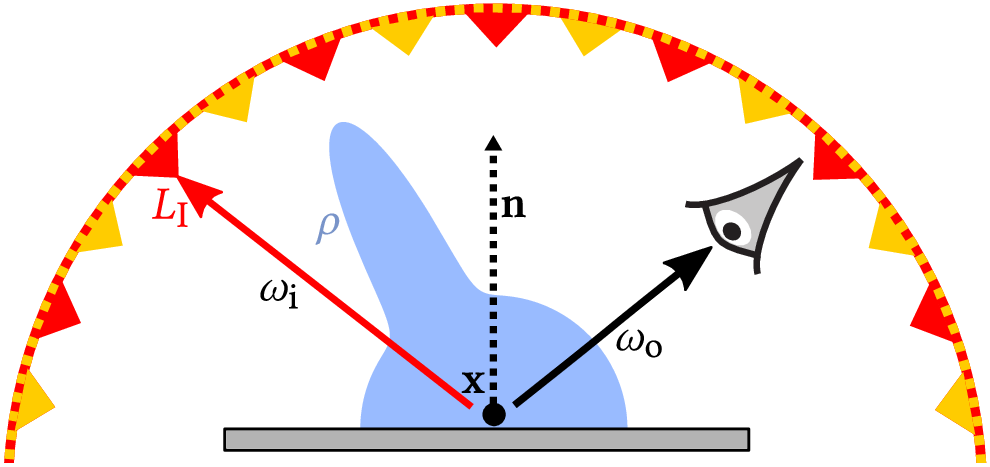
\includegraphics[width=.4\textwidth]{images/ibl_setup.png}
    \caption{Setup for the evaluation of their method.
    Image taken from~\cite[Figure~3]{Karlik2019}.}
    \label{fig:ibl_setup}
\end{figure}

The original pdfs seen in figure~\ref{fig:ibl_pdfs} correspond to the HDR map (in yellow) and the BRDF (in green).

\begin{figure}
    \centering
    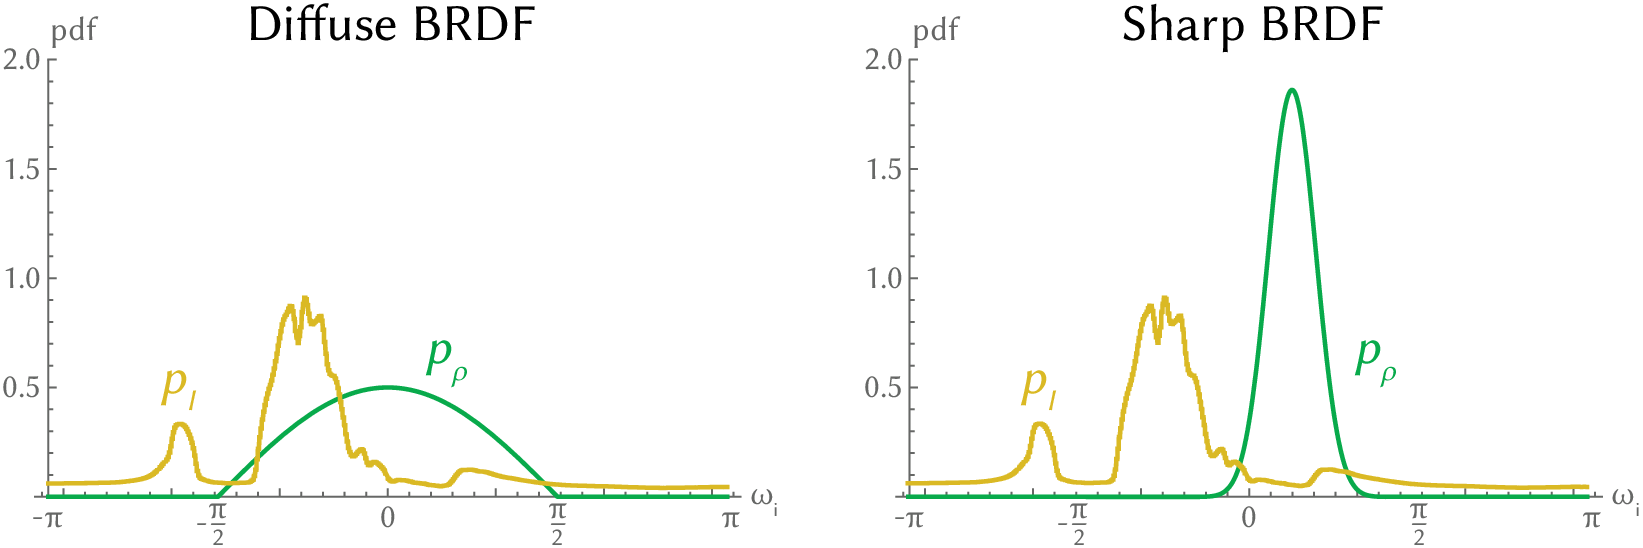
\includegraphics[width=.7\textwidth]{images/ibl_pdfs.png}
    \caption{Original pdfs for the 1D setup.
    The diffuse BRDF corresponds to $ \frac{1}{\pi} $
    whereas the shard BRDF represents a normalized Phong lobe~\cite{phong} with exponent 20 moved by $ \frac{\pi}{8} $ to the right.
    Graphic taken from~\cite[Figure~4]{Karlik2019}}
    \label{fig:ibl_pdfs}
\end{figure}

In figure~\ref{fig:compensated_pdfs} the different pdf they proposed are shown
where the Lagrange multiplier $ \lambda $ was calculated with a \enquote{iterative bisection root-finder within 100 iterations}~\cite[Section~6.3]{Karlik2019}.
The MIS-compensated solution and the optimal one are almost identical with a discrepancy no larger than $ 10^{-5} $
for the mean squared error (MSE) as testes by them in different setups.
The practical pdfs only fit well for the diffuse case, because a diffuse BRDF was assumed in their creation.
Note that the normal-dependent and normal-independent solution are almost the same except for the normal-independent one which has some values for angles outside of $ [ -\frac{\pi}{2}, \frac{\pi}{2} ] $.

\begin{figure}
    \centering
    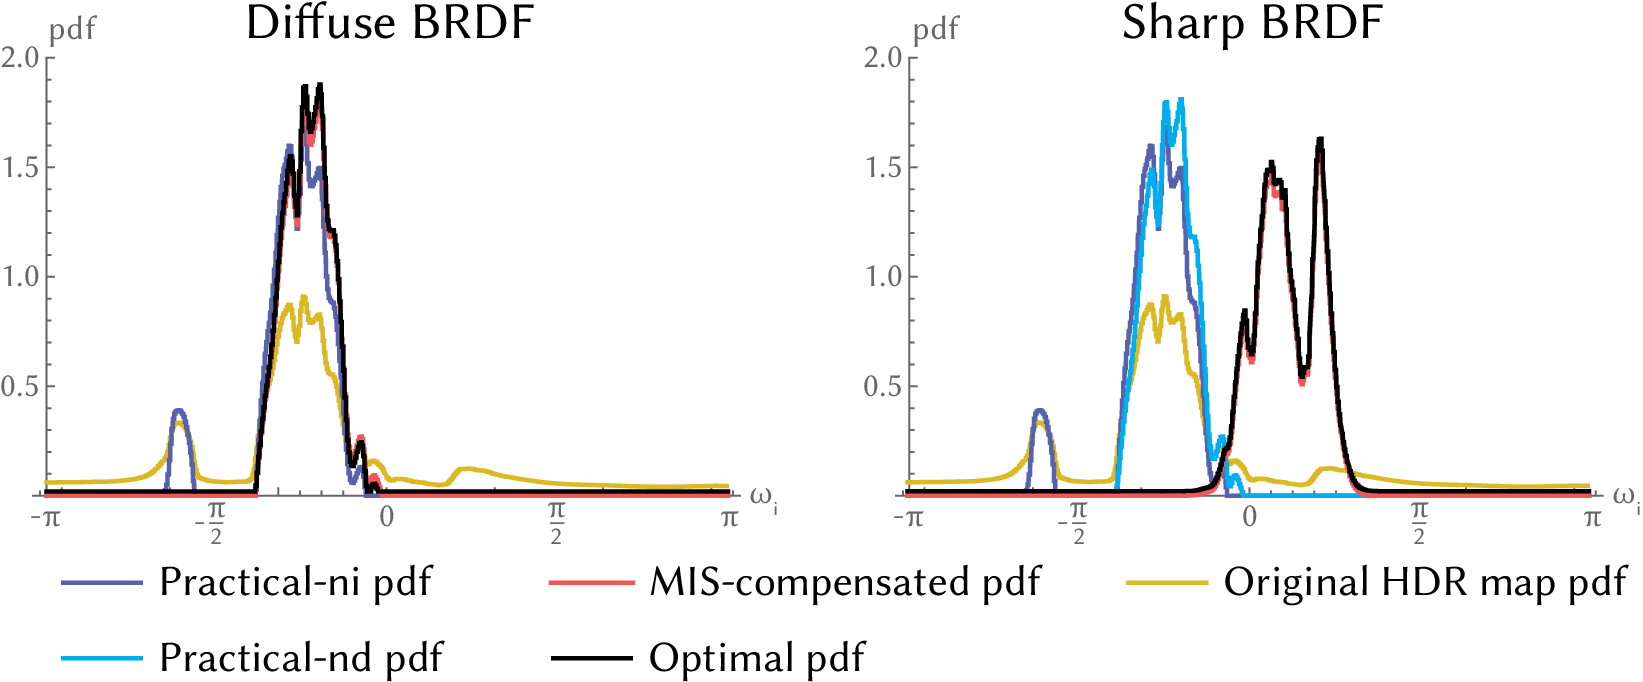
\includegraphics[width=.7\textwidth]{images/ibl_compensated_pdfs.png}
    \caption{Comparison of the different pdfs for the diffuse and sharp BRDF from figure~\ref{fig:ibl_pdfs}.
    Graphic taken from~\cite[Figure~5]{Karlik2019}.}
    \label{fig:compensated_pdfs}
\end{figure}

Figure~\ref{fig:error_plots} shows the MSE of a one-sample and a multi-sample estimator for the diffuse and sharp BRDFs from figure~\ref{fig:ibl_pdfs}.
For the diffuse BRDF of the one-sample estimator sampling from the HDR map compared to standard MIS is almost identical.
Their normal-independent solution is 3.7 times better in regards to the MSE.
The normal-dependent, optimal and compensated pdfs improve the MSE by a factor of 7.5.
For the sharp BRDF the MSE is not improved when using one of the practical pdfs but more importantly it also doesn't worsen it which makes it a good choice compared to standard MIS,
but compared to sampling the BRDF it is worse for a sharp BRDF.
When comparing the optimal solution and the compensated pdf with sampling the BRDF we see an improvement in the MSE by 847 times and compared to regular MIS a 4809 times better MSE.
This shows that there is a lot of potential for better approximations of the compensated pdf.

For the multi-sample estimator the results are similar to the one-sample one,
but note the curve of the practical solutions which are now almost as good as sampling the sharp BRDF,
so even in that case the practical solutions are well suited.
Since the balance heuristic is not the optimal solution for the weights in a multi-sample estimator also the optimal weights~\cite{Kondapaneni2019} are shown,
note that there is still a large discrepancy between the optimal weights and the optimal pdf which suggests that there is hugh potential in finding better pdfs.
The reason why optimal weights can't compete with an optimal pdf is, because no linear combination of the available pdfs is good approximation of the integrand.

\begin{figure}
    \centering
    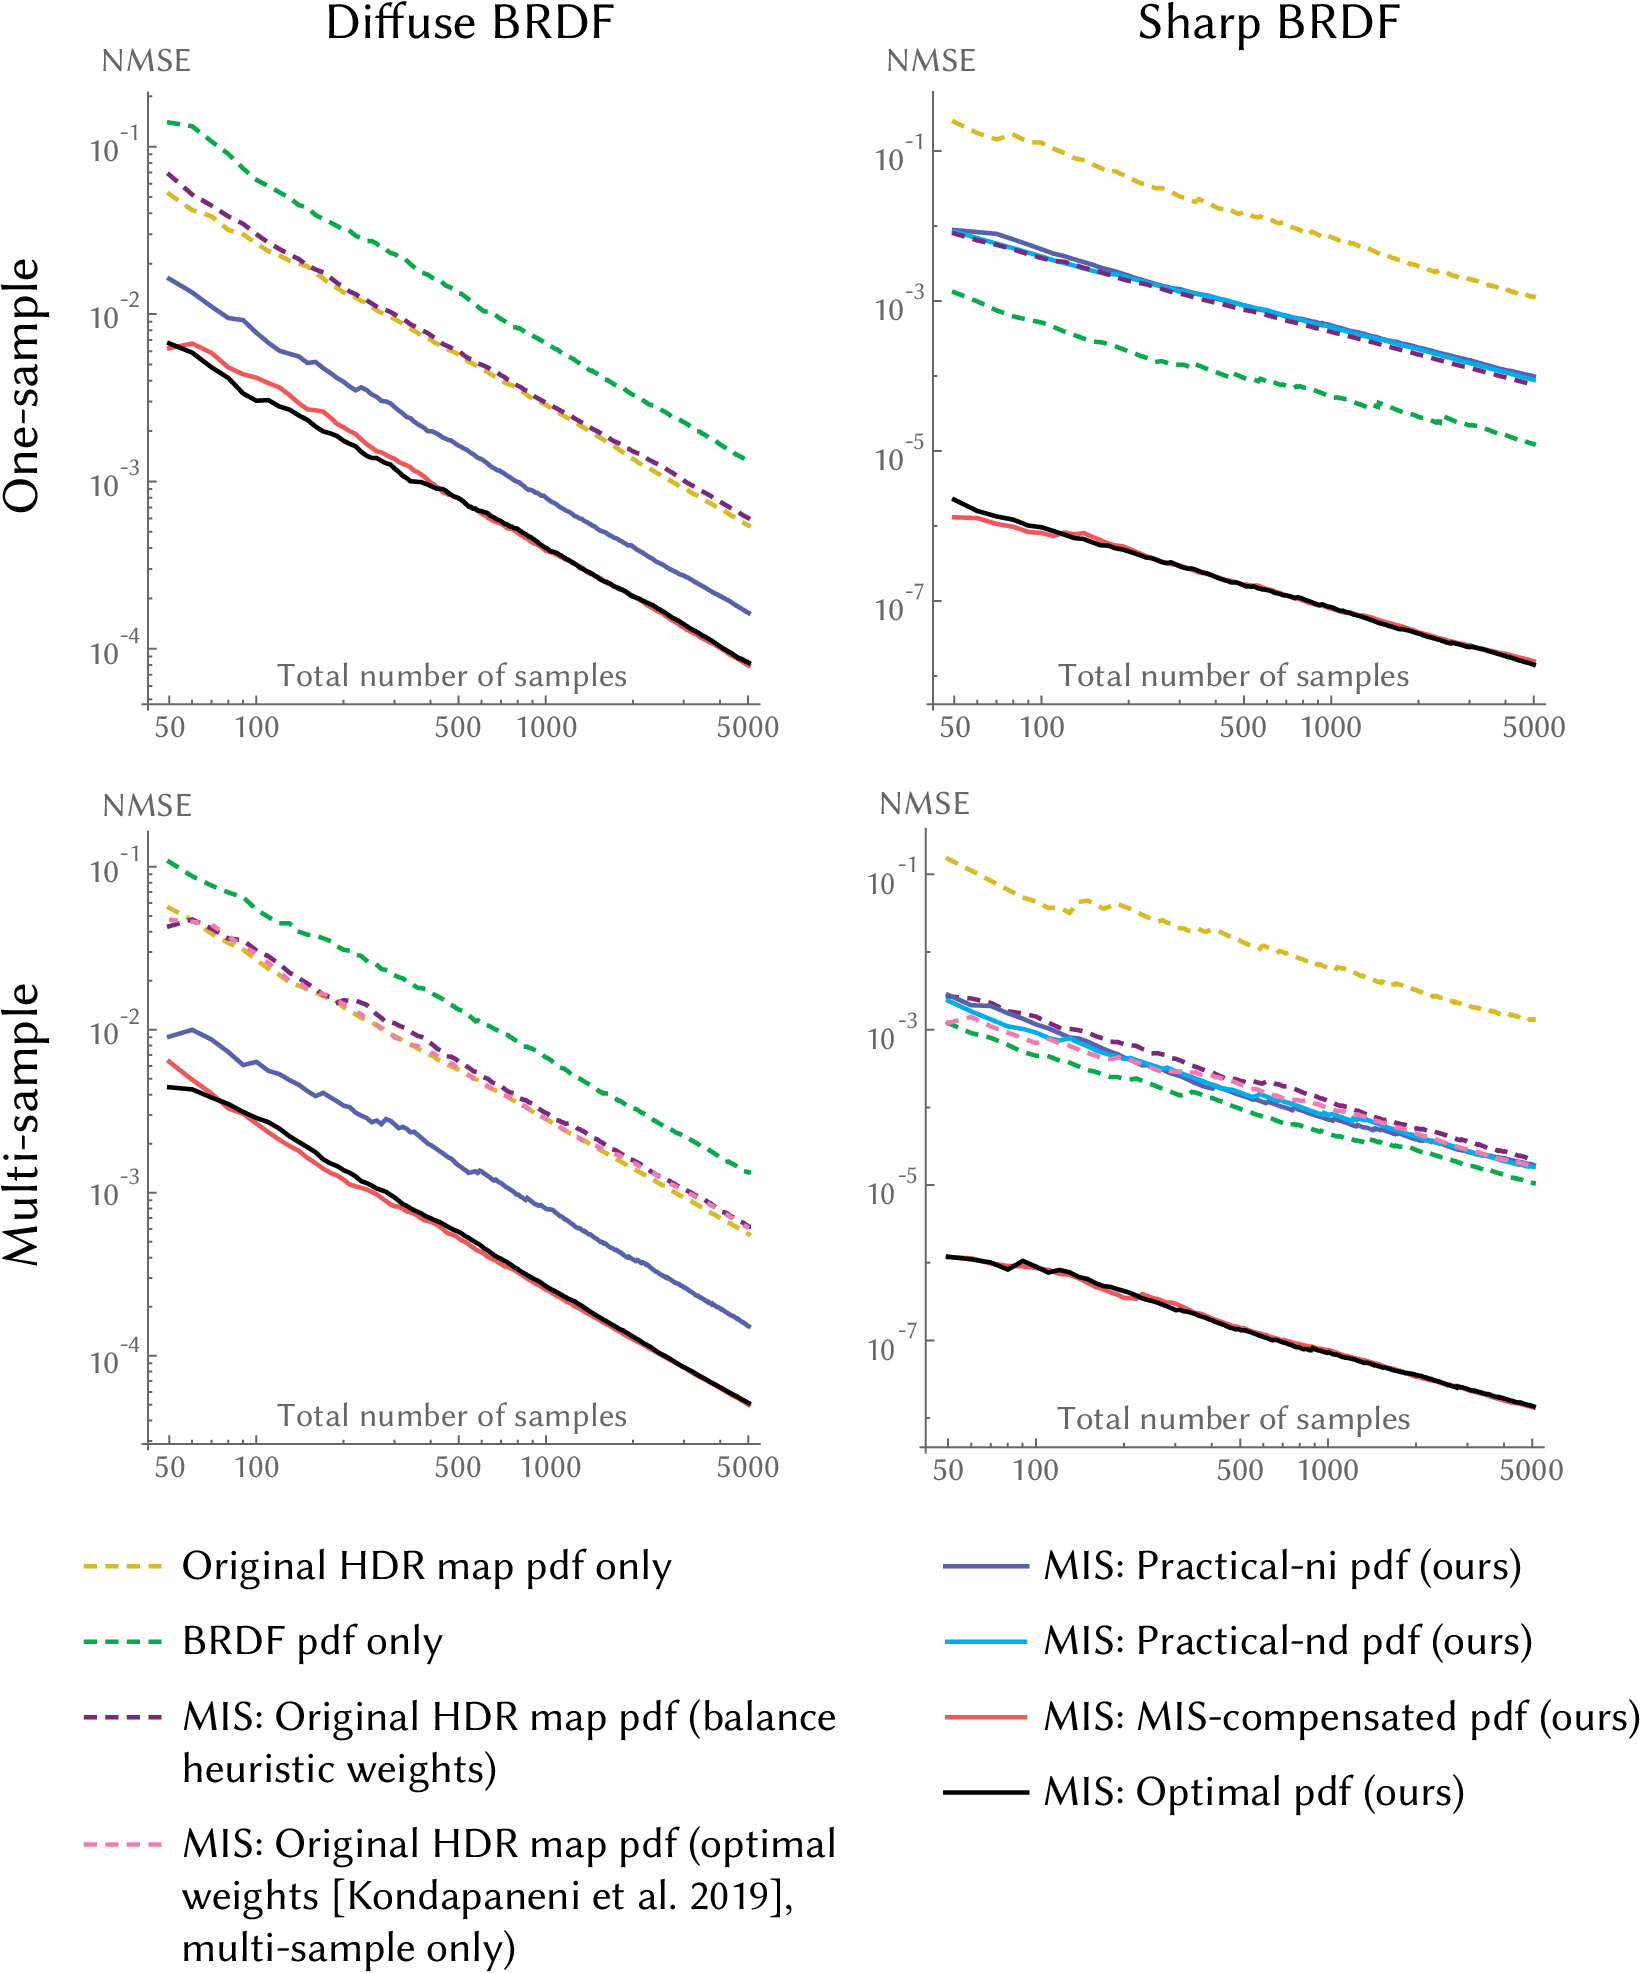
\includegraphics[width=.7\textwidth]{images/error_plots.png}
    \caption{Log-log normalized plot of the MSE for the different estimators.
    The top row shows the results from a one-sample estimator where the bottom row shows the MSE of a multi-sample one.
    In the top row only the balance heuristic is shown as it is provably optimal
    and in the bottom row also the optimal MIS weights from~\cite{Kondapaneni2019} are shown.
    Plots taken from~\cite[Figure~6]{Karlik2019}.}
    \label{fig:error_plots}
\end{figure}

They also did some experiments with real and synthetic scenes to verify their results as can be seen in figure~\ref{fig:sphere_comparison} and~\ref{fig:pills}.
We can see that the variance improvements vanish the lower the contrast of the HDR map becomes and the more specular the object is.
In the Pills scene~\ref{fig:pills} we can clearly see that the compensation reduced the variance noticeably.

\begin{figure}
    \centering
    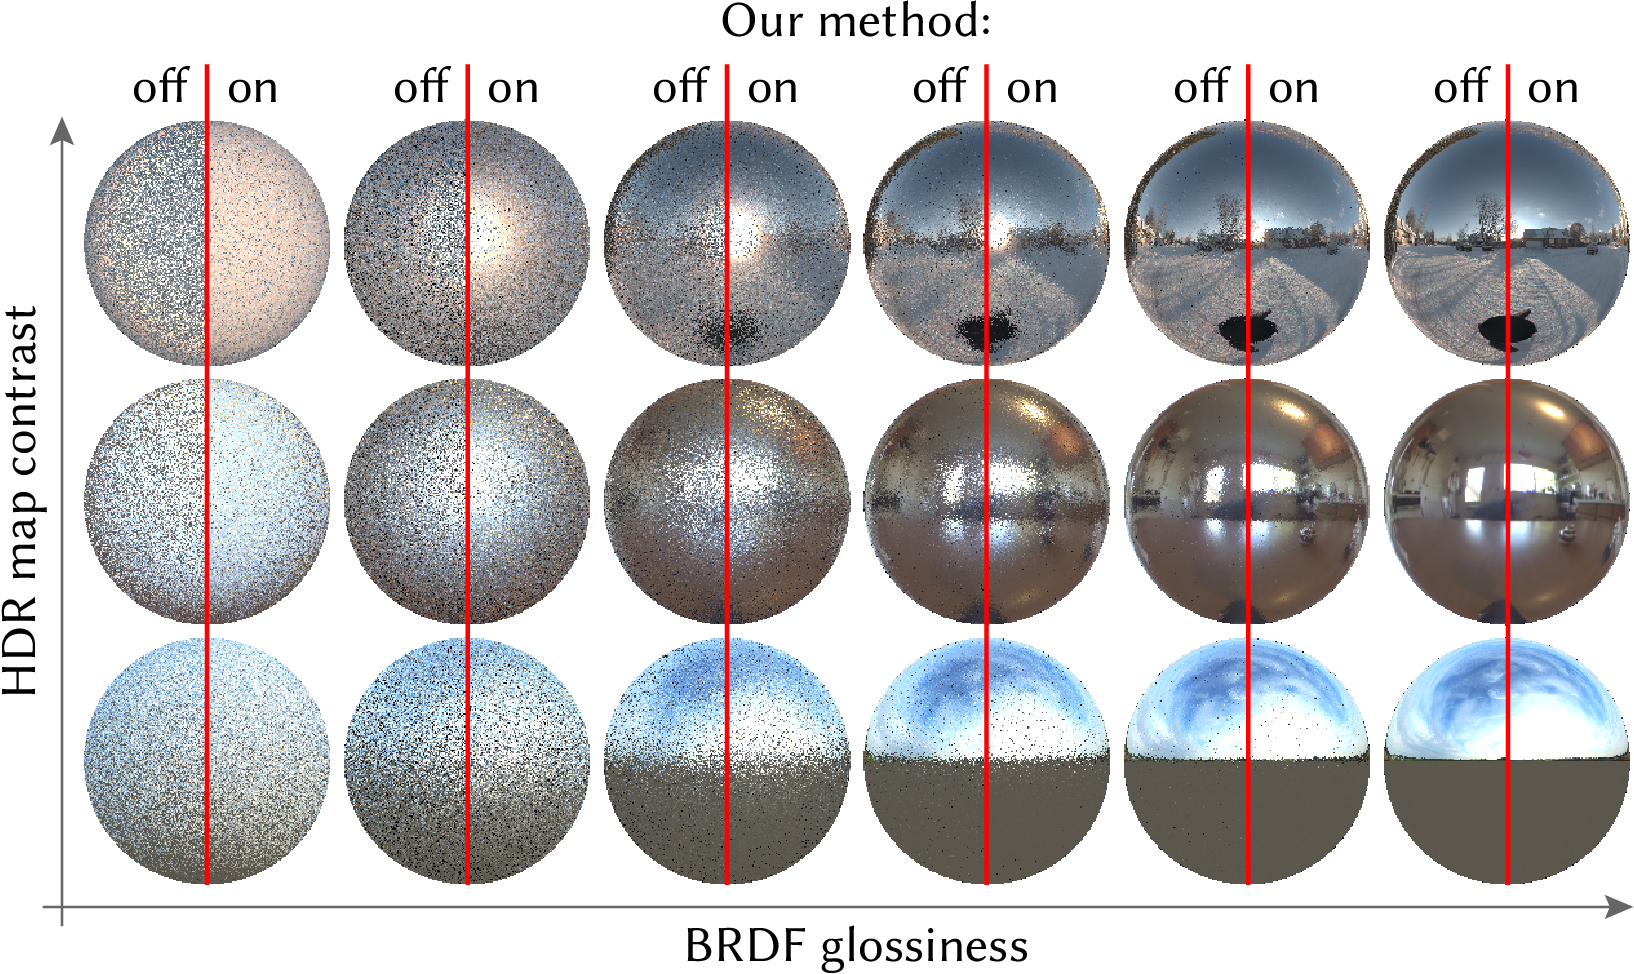
\includegraphics[width=.6\textwidth]{images/sphere_comparison.png}
    \caption{One sample per pixel comparison of rendered spheres with increasing glossiness (from left to right) and HDR map contrast (from bottom to top).
    The left half is rendered with standard MIS and the right half with their normal-independent method.
    Image taken from~\cite[Figure~7]{Karlik2019}}
    \label{fig:sphere_comparison}
\end{figure}

\begin{figure}
    \centering
    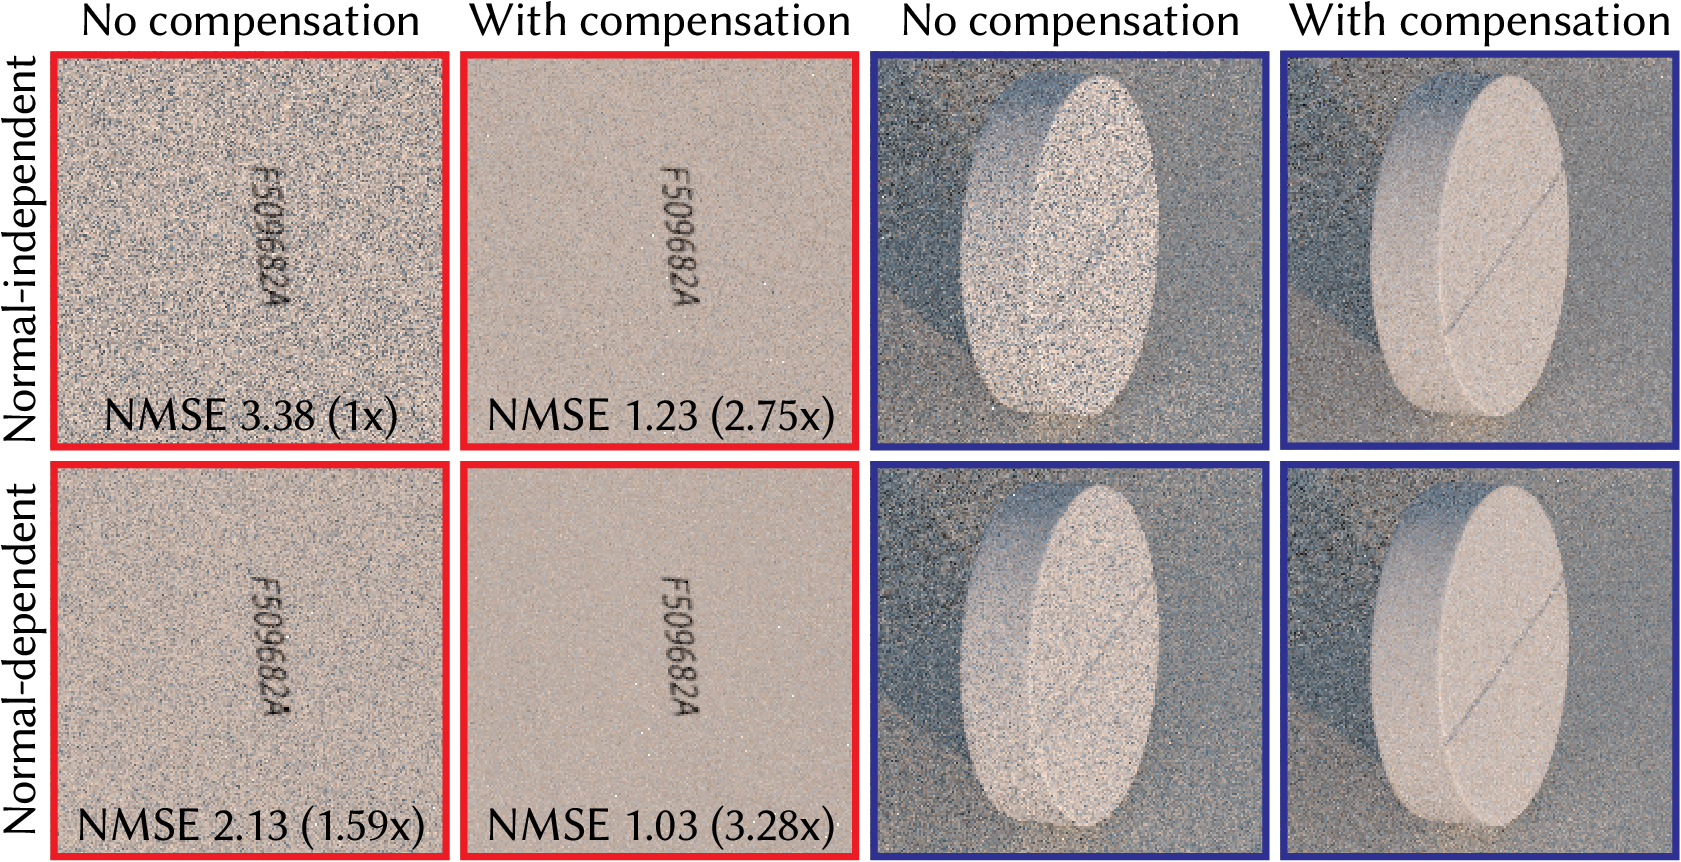
\includegraphics[width=.6\textwidth]{images/pills.png}
    \caption{Equal-time (5s) render of the Pills scene to compare the effect of using MIS compensation with and without normal dependency.
    The normal-independent uncompensated solution show regular MIS
    whereas the normal-dependent uncompensated render shows the effect of premultiplying the HDR map with a diffuse BRDF for each normal direction
    which corresponds to evaluating equation~\ref{eq:normal_dependent} without the subtraction.
    Image taken from~\cite[Figure~9]{Karlik2019}.}
    \label{fig:pills}
\end{figure}